\chapter{Hybrid Hydrogel}\label{chap:2}

% % \chapter*{ }\label{chap:2}
% \addcontentsline{toc}{chapter}{Hybrid Hydrogel}

\begin{figure}[H]
    \centering
    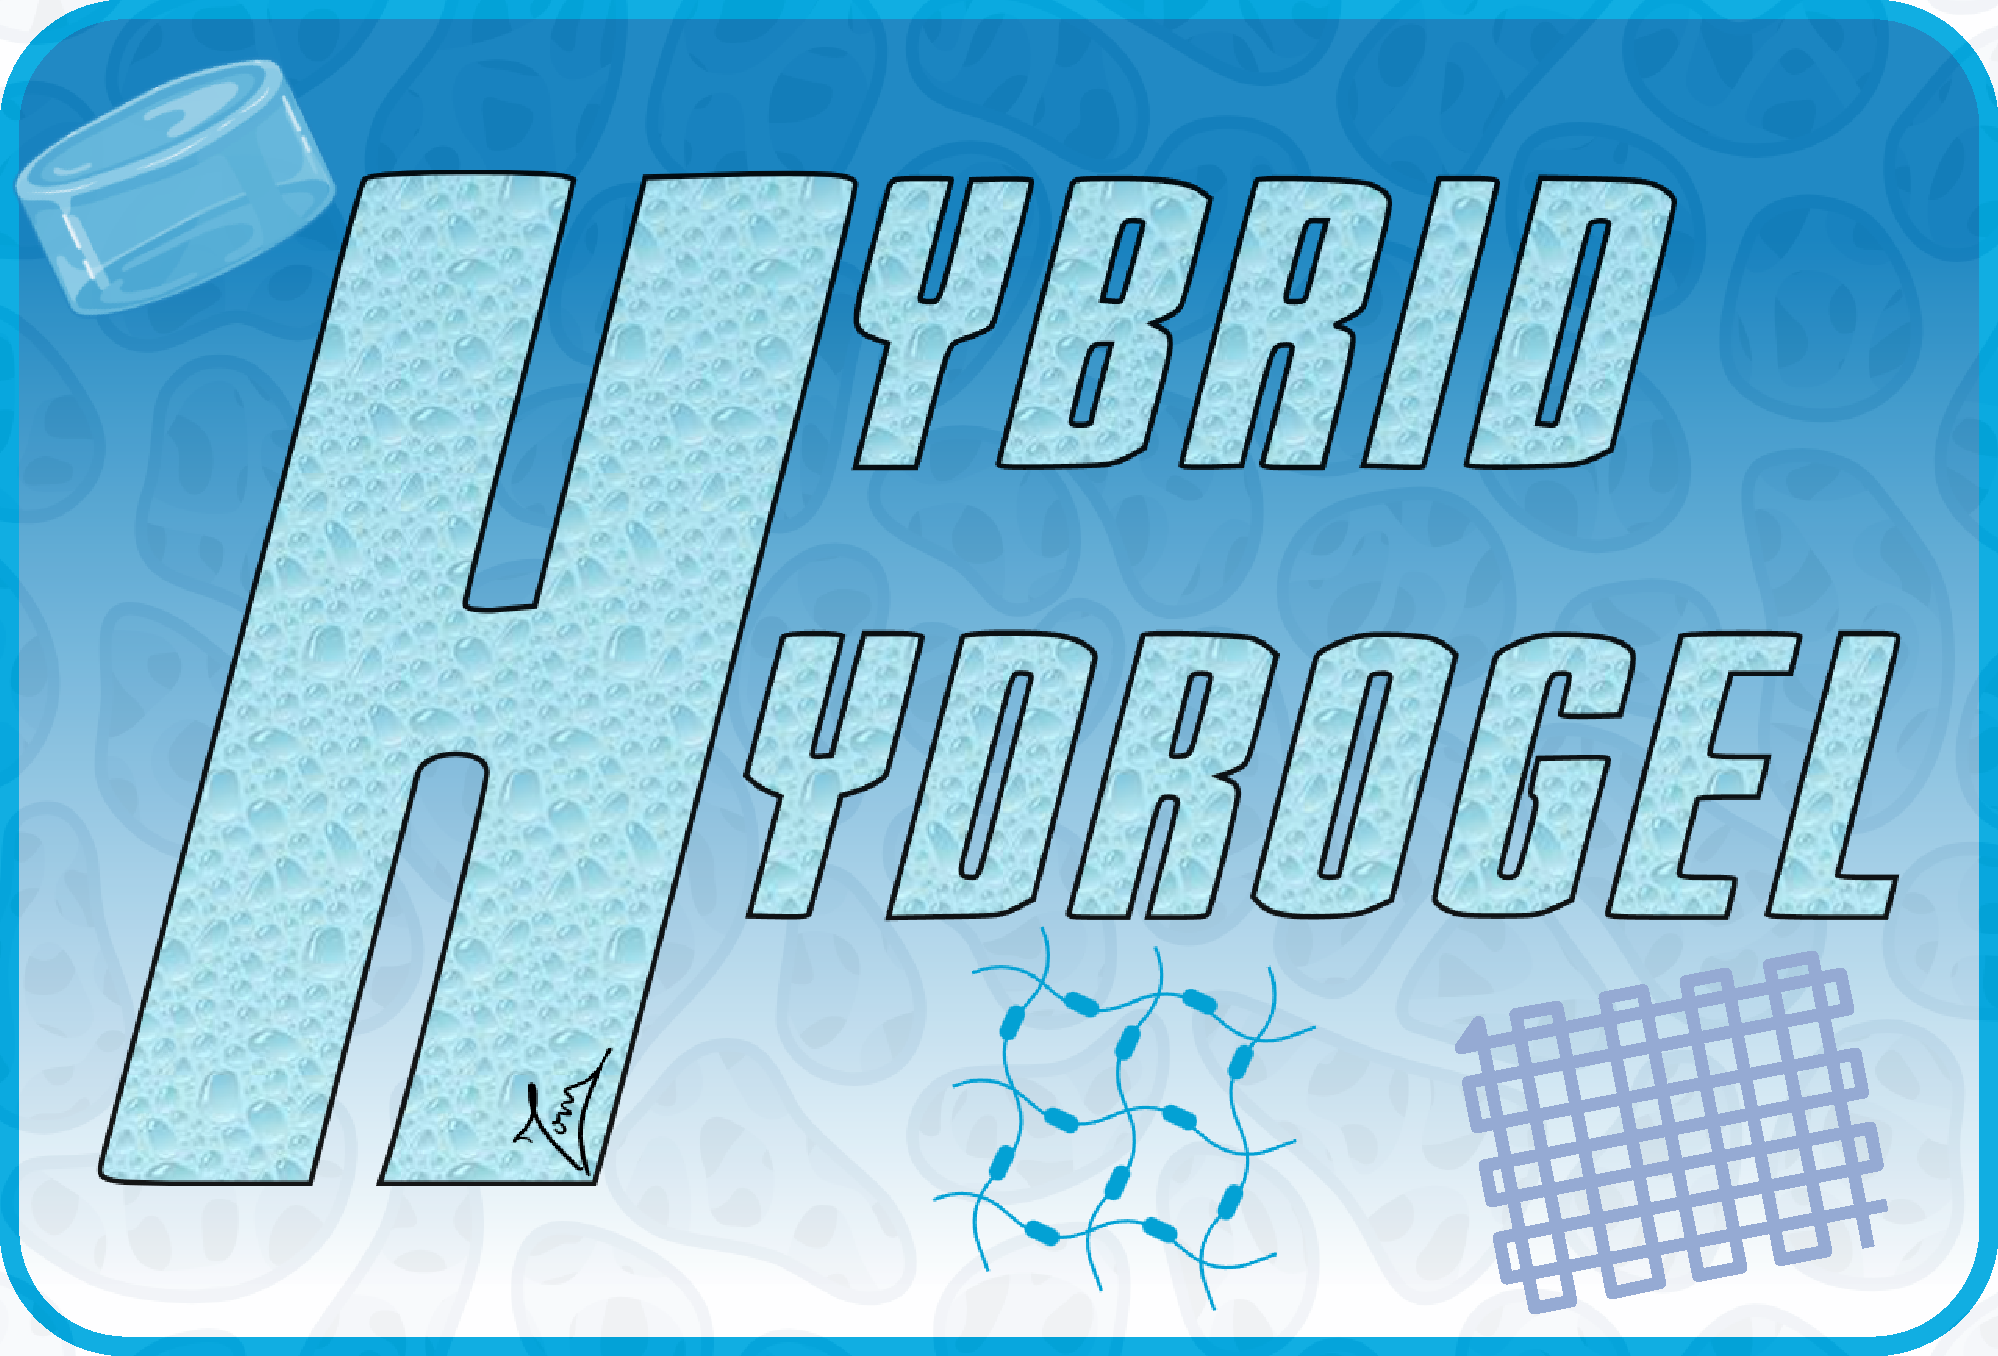
\includegraphics[width=0.85\linewidth]{figures/chapter 2/ch2_hybridhydrogel.pdf}
    \caption[Hybrid Hydrogel Concept]{\textbf{Hybrid Hydrogel Concept.} Hybrid hydrogel concept integrating natural and synthetic components. This chapter introduces the development of a composite hydrogel system designed to mimic the structural and functional characteristics of native meniscal tissue. The hybrid approach combines a hydrated polymer network with synthetic fiber reinforcements, leveraging the biological advantages of natural hydrogels alongside the mechanical robustness of engineered scaffolds. Key aspects include optimizing polymer crosslinking, embedding synthetic meshes, and tailoring the composite architecture to achieve enhanced durability, anisotropy, and cell-instructive properties.}
    \label{fig:ch2_hybridhydrogel}
\end{figure}

\section{Hybrid Design Requirements: \protect\\ Mechanical and Biological Targets}

The development of biomaterials for meniscal tissue engineering requires meeting several critical criteria that span mechanical, biological, and structural domains. The scaffold must exhibit physiologically relevant water content and swelling behavior to maintain the osmotic environment necessary for cellular function. It must possess mechanical properties that enable effective load distribution and stress dissipation under joint loading. Furthermore, it must support cellular adhesion, proliferation, and extracellular matrix production to facilitate biological integration and regeneration. Finally, structural stability under physiological conditions is essential to ensure that the scaffold maintains its form and function during prolonged in vivo use.

\textbf{Water Content and Hydration Behavior.} The target water content of 70--80\% is critical for matching native meniscal tissue characteristics~\cite{morejon2020compressiveproperties}. This hydration level ensures proper osmotic balance within the scaffold, facilitating nutrient diffusion and waste removal while maintaining the viscoelastic properties necessary for load-bearing applications~\cite{chaudhuri2016hydrogelstunable, gu2003newinsight}. The water content directly influences the scaffold's ability to absorb and distribute compressive forces, making it a fundamental parameter for successful meniscal replacement.

\textbf{Matrix Distribution and Solid-to-Fluid Ratios.} Strategic PCL integration must maintain appropriate solid-to-fluid ratios that balance mechanical reinforcement with biological functionality~\cite{elkommos2025hybridhydrogels, fares2018interpenetratingnetwork}. The synthetic component provides structural integrity and load-bearing capacity, while the hydrogel matrix preserves the hydrated environment essential for cellular activity. This balance is crucial for creating scaffolds that can withstand physiological loading while supporting tissue regeneration and integration.

\textbf{Regional Variation and Tissue Organization.} Composition gradients mimicking native tissue organization are essential for replicating the meniscus's anisotropic mechanical properties~\cite{bahcecioglu20193dprinted, du2023meniscusheterogeneity, bulle2021humanmeniscus}. The native meniscus exhibits region-specific variations in collagen fiber orientation, proteoglycan content, and mechanical stiffness that correspond to different functional demands. Scaffolds must incorporate similar gradients to ensure proper load distribution and stress dissipation across the entire tissue construct.

\textbf{Structural Stability and Physiological Loading.} Maintenance of form under physiological loading conditions is paramount for long-term scaffold performance~\cite{bilgen2018currentconcepts, ghodbane2019partialmeniscus}. The meniscus experiences complex loading patterns including compression, tension, and shear forces during normal joint function. Scaffolds must demonstrate sufficient structural integrity to resist deformation and degradation under these conditions while maintaining their biological functionality throughout the healing process.

Given these requirements, natural or composite natural--synthetic biomaterials offer a promising solution. The meniscus's highly organized fibrocartilaginous structure, responsible for absorbing dynamic compressive loads and dissipating mechanical stress within the knee joint, demands scaffolds that can replicate both its mechanical and biological behavior. The integration of natural hydrogels with synthetic reinforcements provides a pathway to achieve these competing demands, enabling the development of biomaterials that combine the biological advantages of natural polymers with the mechanical robustness of engineered materials.

\textbf{Natural-Synthetic Material Integration Strategy.} To address the competing demands of biological functionality and mechanical performance, our approach leverages the complementary properties of natural and synthetic biomaterials. Natural materials, specifically gelatin A (GelA) derived from porcine collagen, provide essential biological cues including cell-binding motifs and inherent biocompatibility that support cellular adhesion, proliferation, and extracellular matrix production~\cite{ahmed2015hydrogelpreparation, zhang2005electrospinninggelatin}. These natural components maintain the hydrated environment necessary for cellular function while offering tunable mechanical properties through controlled crosslinking~\cite{chaudhuri2016hydrogelstunable}.

Conversely, synthetic materials such as polycaprolactone (PCL) provide the structural integrity and load-bearing capacity required for meniscal applications~\cite{woodruff2010returnforgotten, gao2018electrospunfiber}. PCL's excellent mechanical properties, including high tensile strength and elongation at break, enable scaffolds to withstand the complex loading patterns experienced in the knee joint. The synthetic component also offers predictable degradation kinetics and processing versatility, allowing for precise control over scaffold architecture and mechanical reinforcement patterns~\cite{field2021tuneablephotocurable}.

The strategic integration of these materials creates a hybrid system where the natural hydrogel component maintains biological functionality while the synthetic reinforcement network provides mechanical stability. This approach enables the development of scaffolds that can meet the water content requirements (70--80\%) while simultaneously achieving the mechanical properties necessary for load-bearing applications~\cite{elkommos2025hybridhydrogels}. The resulting composite materials demonstrate enhanced structural stability under physiological conditions while preserving the biological environment essential for tissue regeneration and integration.

\begin{figure}[H]
    \centering
    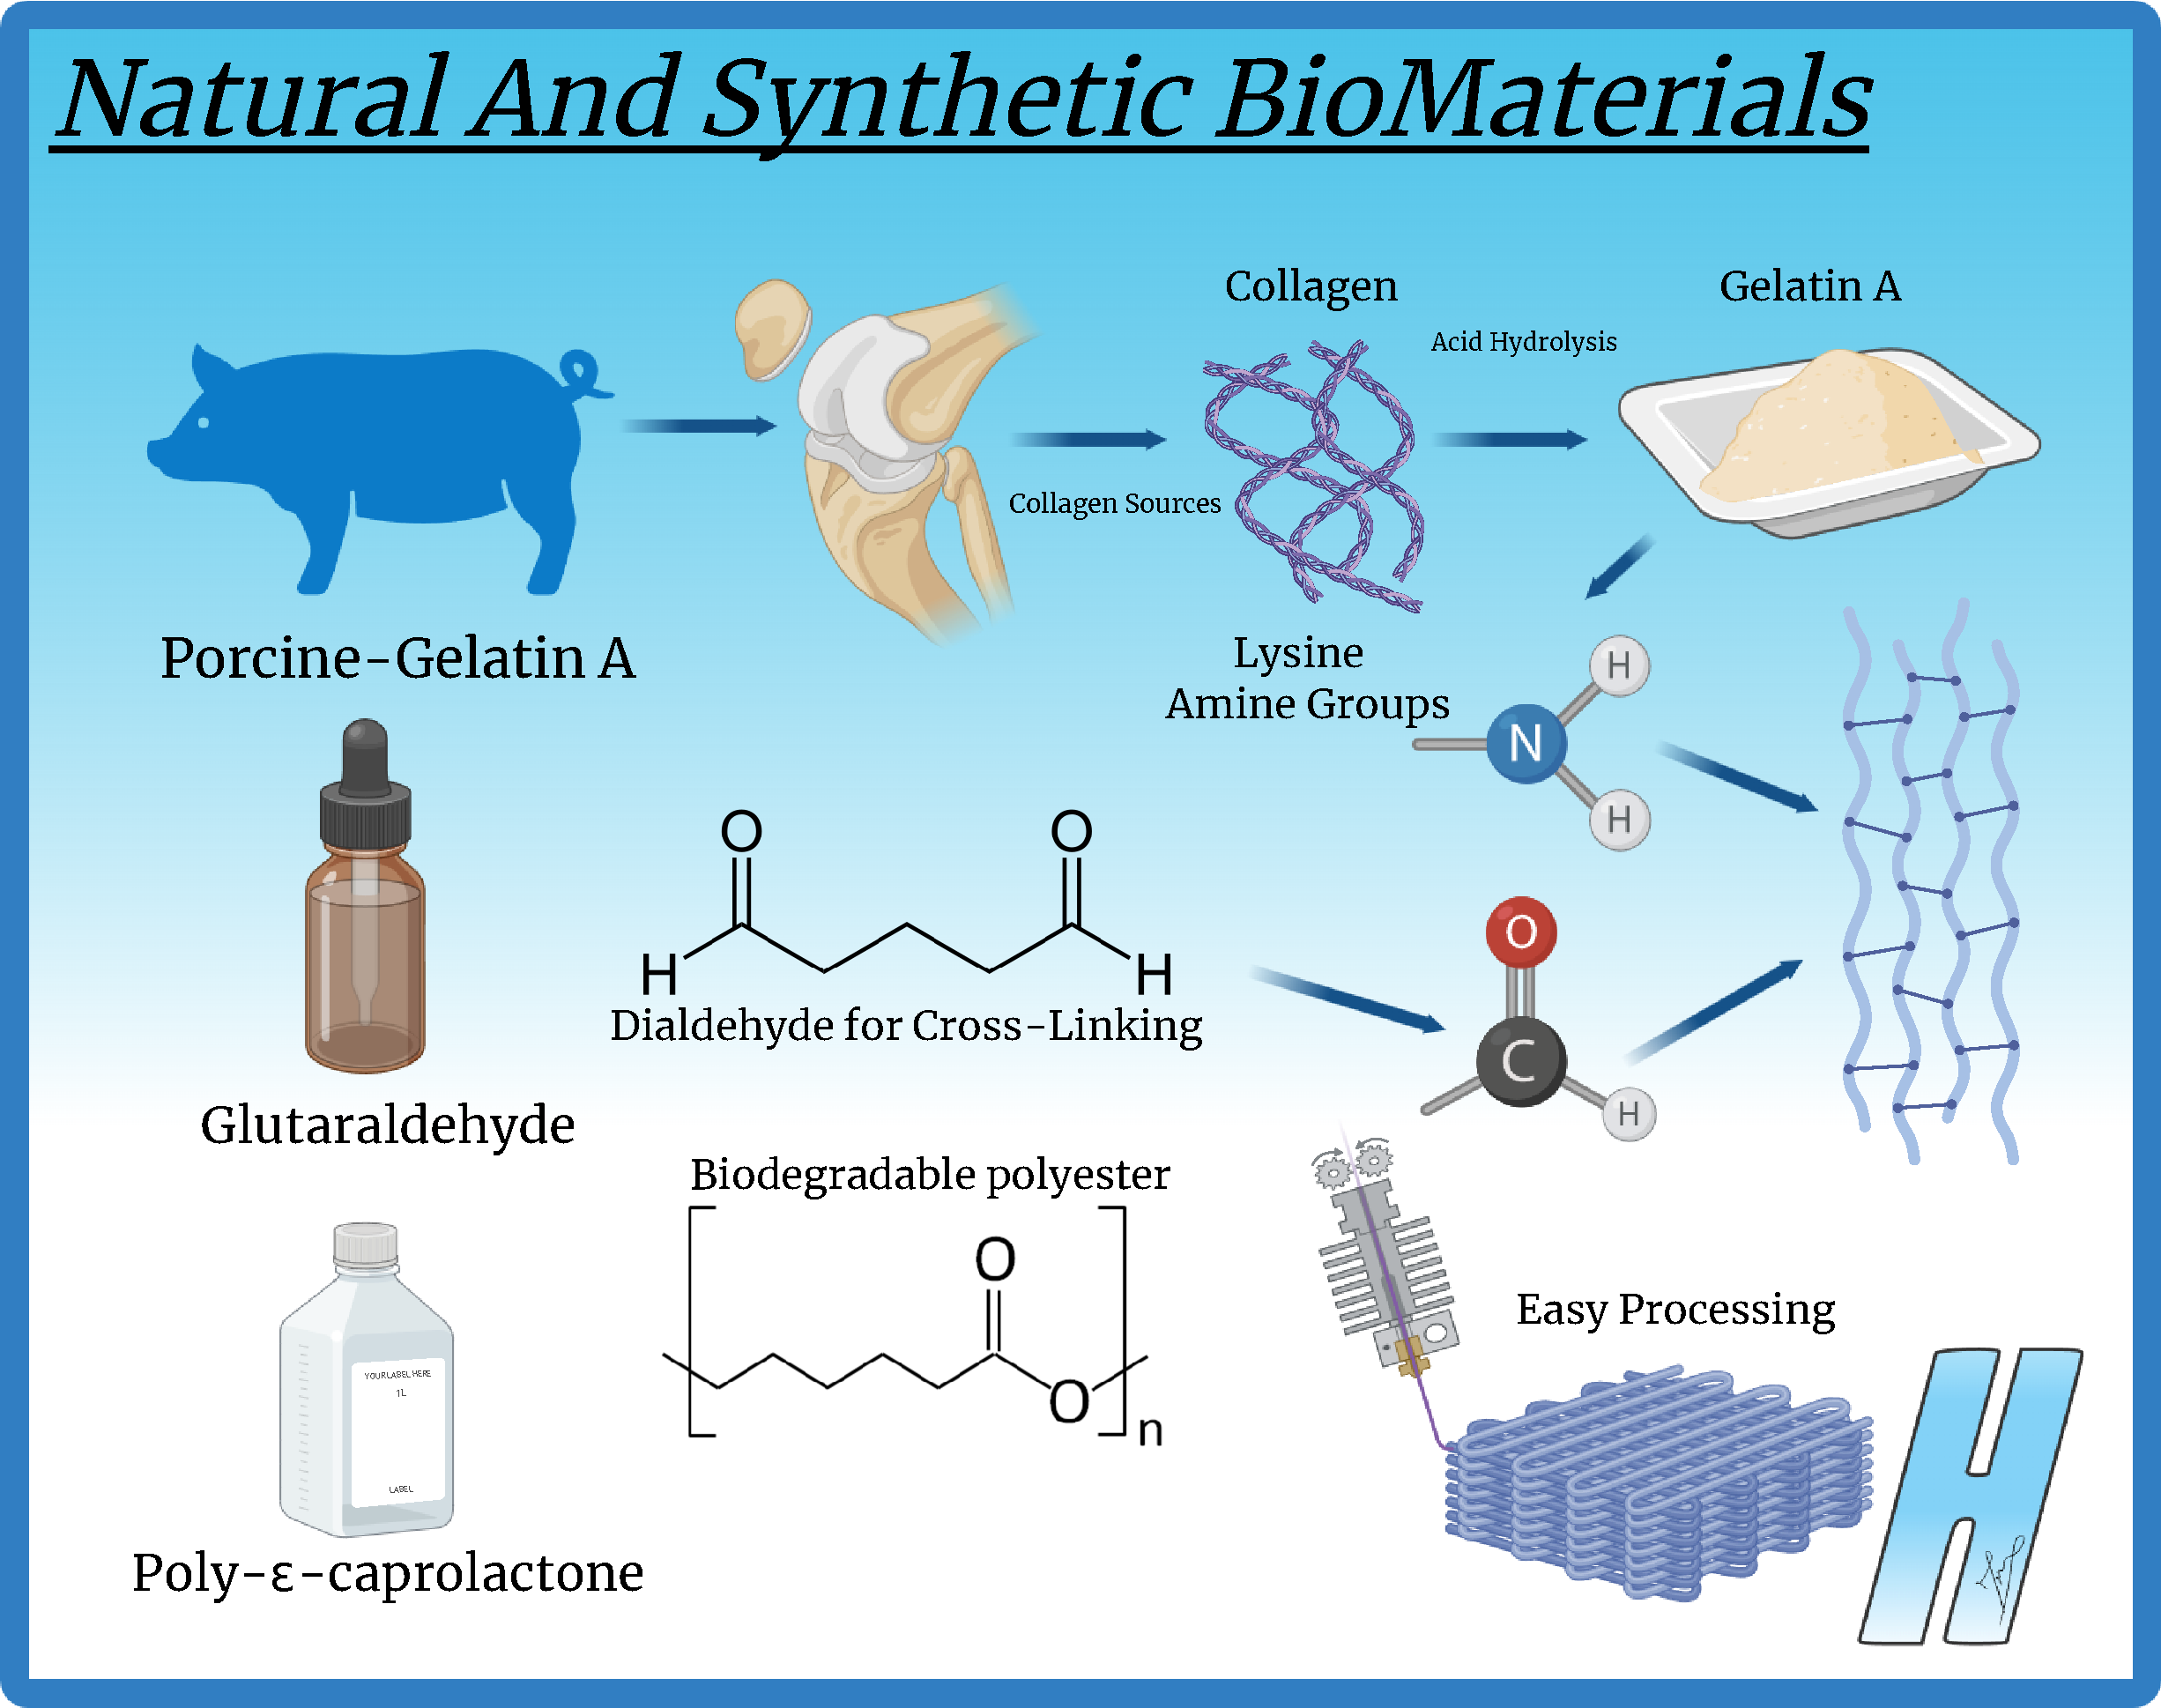
\includegraphics[width=0.85\linewidth]{figures/chapter 2/ch2_biomaterials.pdf}
    \caption[Overview of Natural and Synthetic Biomaterials Used in Scaffold Fabrication]{\textbf{Overview of Natural and Synthetic Biomaterials Used in Scaffold Fabrication.} Porcine-derived gelatin A (GelA) is obtained through acid hydrolysis of collagen, preserving lysine amine groups essential for crosslinking. Glutaraldehyde (GTA), a dialdehyde crosslinker, facilitates network formation by reacting with amine groups on GelA chains. Poly-$\varepsilon$-caprolactone (PCL), a biodegradable polyester, serves as a synthetic reinforcement material, offering mechanical strength and ease of processing for composite scaffold integration. }
    \label{fig:ch2_biomaterials}
\end{figure}

\clearpage
\subsection{Polycaprolactone Integration: Mechanical Reinforcement and Biocompatibility}

While GelA-based hydrogels provide excellent biological properties and tunable swelling behavior, they often lack the mechanical strength required for load-bearing applications such as meniscal replacement~\cite{2021synthesisapplication}. To address this limitation, polycaprolactone (PCL) was integrated as a synthetic reinforcement component~\cite{bagherisaed2020functionalizedpoly}. PCL is a biodegradable aliphatic polyester with excellent mechanical properties, long-term structural stability, and established biocompatibility in orthopedic applications~\cite{woodruff2010returnforgotten, pitt1981aliphaticpolyesters}.
The integration of PCL reinforcement networks within the GelA hydrogel matrix creates a hybrid scaffold system that leverages the complementary properties of both materials. PCL provides mechanical strength and structural integrity, while the GelA hydrogel component maintains the physiological water content and biological signaling necessary for cellular function. This hybrid approach enables the development of composite scaffolds that better mimic the complex mechanical behavior of native meniscal tissue~\cite{zhang20173dprintedpolyecaprolactone, yang2016multilayeredpolycaprolactone}.

The role of PCL in mechanical reinforcement and its integration with GelA hydrogels will be explored in detail in subsequent sections, particularly as we examine the development of Hybrid Hydrogels Augmented via Network Integration (HANI) biomaterials~\cite{elkommos2025hybridhydrogels}. This systematic investigation will demonstrate how PCL networks can be strategically incorporated to enhance mechanical properties while maintaining the beneficial biological characteristics of the GelA matrix~\cite{zhang20173dprintedpolyecaprolactone, yang2016multilayeredpolycaprolactone}.

PCL exhibits excellent mechanical characteristics including a Young's modulus of 300-400 MPa and tensile strength of 10-25 MPa, with high elongation at break (300-500\%)~\cite{woodruff2010returnforgotten, pitt1981aliphaticpolyesters}. The material's biodegradability occurs over months to years through hydrolytic ester cleavage~\cite{gao2018electrospunfiber}, with demonstrated biocompatibility through FDA-approved medical devices~\cite{gautam2013fabricationcharacterization, zhang2005electrospinninggelatin}.

\begin{table}[H]
    \centering
    \caption[PCL Material Properties.]{\textbf{PCL Material Properties.} Data adapted from Woodruff et al. \cite{woodruff2010returnforgotten}, Pitt et al. \cite{pitt1981aliphaticpolyesters}, and Gunatillake et al. \cite{gunatillake2003biodegradablepolymers}.}
    \label{tab:PCL-properties}
    \renewcommand{\arraystretch}{1.3}
    \setlength{\tabcolsep}{12pt}
    \begin{tabular}{|p{4.5cm}|p{4cm}|}
        \hline
        \cellcolor{blue!20}\textbf{Property} & \cellcolor{blue!20}\textbf{Value} \\[0.3em]
        \hline
        Molar mass (monomer) & 114.14 g/mol \\[0.3em]
        \hline
        Density & 1.145--1.150 g/cm$^3$ \\[0.3em]
        \hline
        Melting point & 58--63$^\circ$C \\[0.3em]
        \hline
        Glass transition temperature (Tg) & --60$^\circ$C \\[0.3em]
        \hline
        Crystallinity & 45--65\% \\[0.3em]
        \hline
        Young's modulus & 300--400 MPa \\[0.3em]
        \hline
        Tensile strength & 10--25 MPa \\[0.3em]
        \hline
        Elongation at break & 300--500\% \\[0.3em]
        \hline
        Flexural modulus & $\sim$400 MPa \\[0.3em]
        \hline
        Decomposition temperature & $\sim$350$^\circ$C \\[0.3em]
        \hline
        Biodegradability & Months to years \\[0.3em]
        \hline
        Biocompatibility & Excellent \\[0.3em]
        \hline
        Degradation byproduct & Caproic acid \\[0.3em]
        \hline
    \end{tabular}
\end{table}




\subsection{Gelatin A: \protect\\ Biochemical Properties and Mechanical Contributions}

Gelatin Type A (hereafter GelA), a hydrolyzed form of collagen, was selected as the base material for hydrogel fabrication~\cite{ahmed2015hydrogelpreparation}. Derived from type I collagen, GelA provides inherent biocompatibility, biodegradability, and the presence of cell-binding motifs such as Lys-Arg-Gly-Asp (L-RGD) sequences, promoting cellular adhesion, proliferation, and differentiation~\cite{2021synthesisapplication,ahmed2015hydrogelpreparation,choi20213dprintedgelatin,zhang2005electrospinninggelatin}. These attributes are critical for supporting fibrocartilaginous matrix deposition and maintaining cellular activity within engineered scaffolds. Additionally, GelA's mechanical properties are tunable via polymer concentration and crosslinking density, allowing the fabrication of hydrogels that mimic the viscoelastic characteristics of the native meniscus.

Extensive research supports the use of GelA as a scaffold material in cartilage and meniscal tissue engineering. Studies have demonstrated that GelA-based constructs promote better cell attachment and extracellular matrix production compared to alternatives like alginate and chitosan, which lack intrinsic cell-binding motifs. Furthermore, GelA's ability to undergo various crosslinking reactions enables precise mechanical property tuning to better match the biomechanical environment of the knee.

\subsection{Glutaraldehyde Crosslinking: \protect\\ Chemical Mechanisms and Property Control}

While GelA offers significant biological advantages, its structural integrity at physiological temperatures is poor, leading to rapid degradation and mechanical failure. To enhance stability and extend functional performance, chemical crosslinking is required~\cite{ahmed2015hydrogelpreparation,gao2018electrospunfiber,chaudhuri2016hydrogelstunable}. Crosslinking introduces covalent bonds between GelA chains, creating a stable network that can resist enzymatic degradation and mechanical forces within the joint environment.

Glutaraldehyde (GTA) was selected as the crosslinking agent due to its ability to form stable covalent bonds between free amine groups in the GelA matrix. GTA crosslinking effectively increases the hydrogel's mechanical stiffness, improves structural stability, and allows tuning of water content and degradation rates. However, the potential cytotoxicity of residual GTA necessitates rigorous post-crosslinking rinsing protocols. In this study, all hydrogels underwent extensive rinsing and equilibration to remove unreacted GTA, ensuring biocompatibility while maintaining mechanical performance.

\section{Hydrogel Development Strategy and Methodology} \label{sec:ch2_methods}

\subsection{Gelatin-GTA Hydrogel Fabrication Overview}
Hydrogel fabrication was performed through a systematic crosslinking protocol involving GelA solutions and varying concentrations of GTA. Solutions were cast into defined molds, crosslinked under controlled conditions, thoroughly rinsed to remove unreacted crosslinker, and equilibrated in phosphate-buffered saline (PBS) to achieve osmotic balance. This standardized fabrication process enabled reproducible hydrogel properties across experimental groups, facilitating systematic evaluation of how crosslinking parameters influence swelling behavior, mechanical properties, and stress-relaxation characteristics.

\subsection{Gelatin Hydrogel Preparation}

Gelatin-based hydrogels were fabricated using Type A gelatin (300 bloom, Sigma-Aldrich) with precise temperature and pH control. The 0.15 g/mL GelA solution was prepared at 65$^\circ$C under continuous stirring (400 rpm) to ensure complete solubilization. Solution pH was maintained at 7.4 ± 0.1 using PBS buffer to optimize crosslinking conditions. Glutaraldehyde (GTA) stock solution (25\%, Sigma-Aldrich), diluted to specific concentrations (v/v) in PBS, was then added at various volumes to the GelA solution.

The resulting hydrogel precursor solutions were cast into custom-designed molds and allowed to crosslink at room temperature (23\textdegree C) for 1 hour. Crosslinking was terminated by briefly immersing the hydrogels in PBS for 5 minutes, followed by an equilibration step in PBS at 4\textdegree C for 12 hours to ensure full osmotic balance prior to further characterization.

\begin{figure}[H]
    \centering
    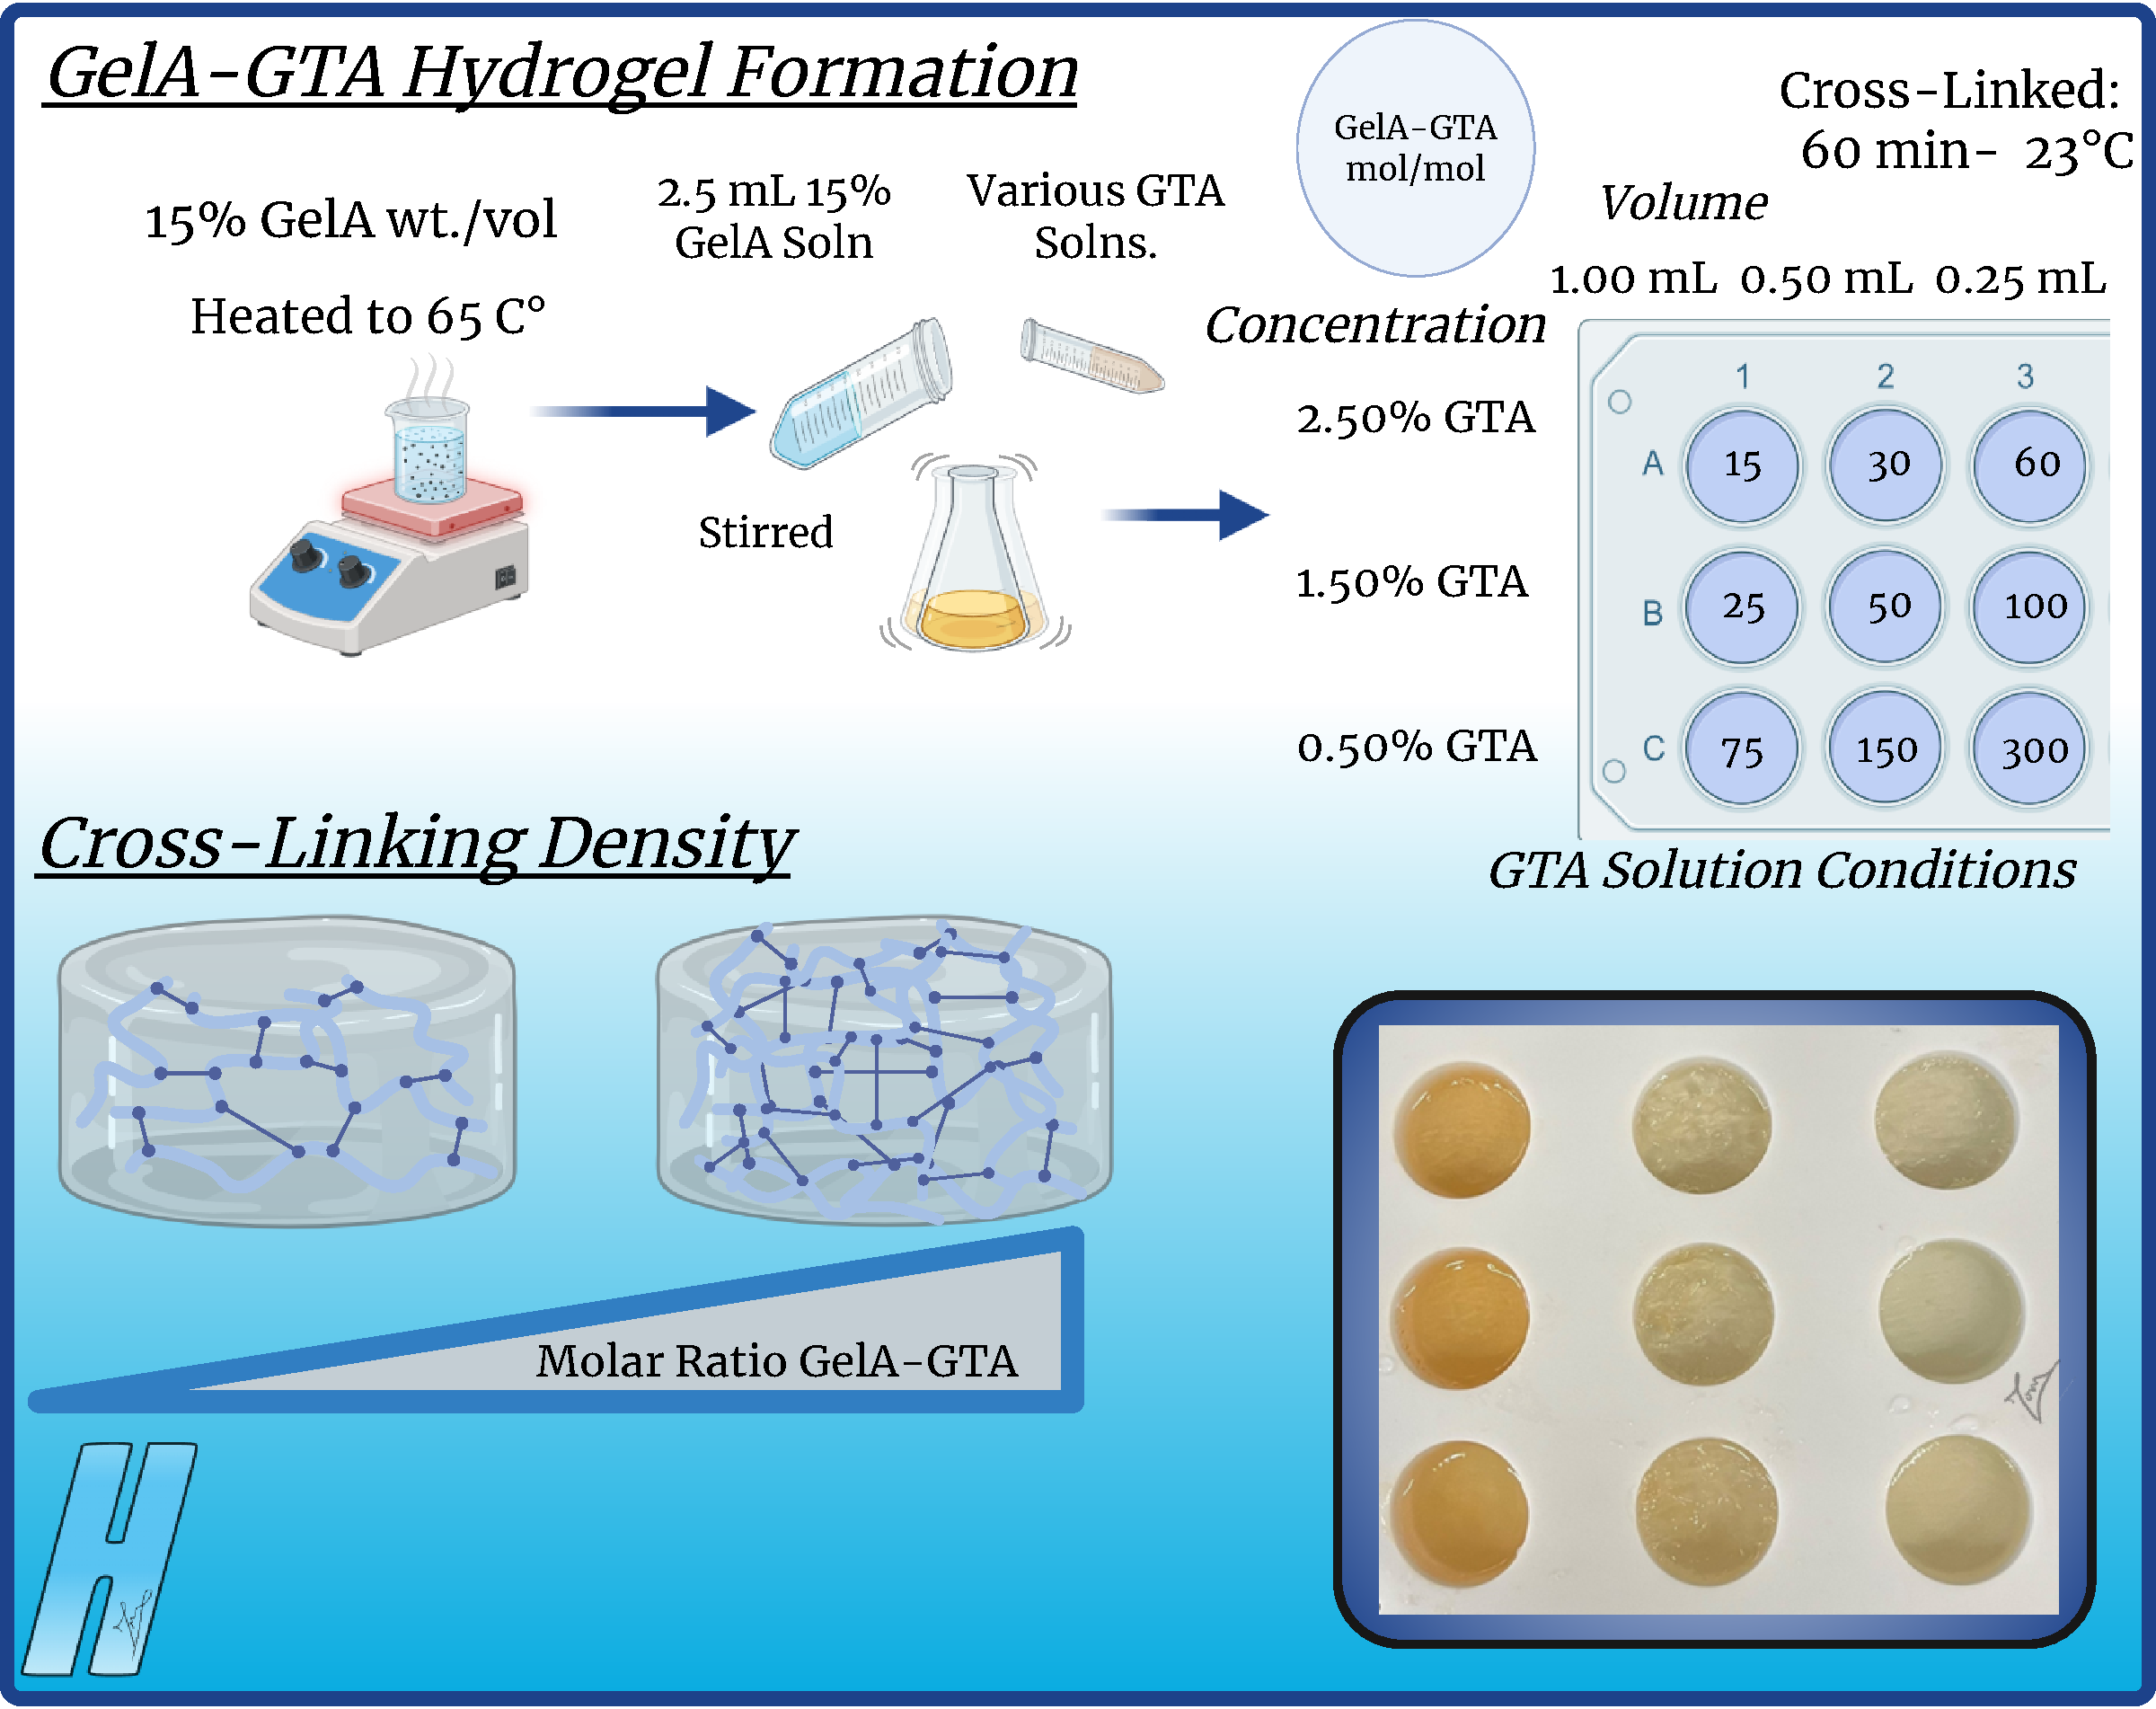
\includegraphics[width=0.85\linewidth]{figures/chapter 2/ch2_hydrogel.pdf}
    \caption[GelA--GTA Hydrogel Fabrication and Crosslinking Behavior]{\textbf{GelA--GTA Hydrogel Fabrication and Crosslinking Behavior.} Schematic overview of hydrogel synthesis using 15\% (w/v) GelA solution crosslinked with glutaraldehyde (GTA) at varying concentrations (0.5\%, 1.5\%, 2.5\% v/v) and crosslinker volumes (0.25, 0.50, and 1.00 mL). The hydrogels were formed by heating to 65°C and stirring prior to crosslinking at room temperature (23°C) for 60 minutes. The crosslinking density (bottom left) illustrates increasing network tightness with rising GTA molar ratios. The GTA solution matrix (top right) highlights different solution conditions used for crosslinking. The photographic comparison (bottom right) shows hydrated hydrogels post-fabrication, demonstrating variations in physical appearance across formulations, with 0.5\% and 1.5\% GTA at 0.25 mL achieving hydration profiles approximating native meniscal water content. }
    \label{fig:ch2_hydrogel}
\end{figure}

\subsection{Crosslinking Concentrations and Volumes}

To systematically explore the effects of crosslinking density, nine hydrogel groups were prepared by varying the GTA concentration (0.5\%, 1.5\%, and 2.5\% v/v) and crosslinker volume (0.25, 0.50, and 1.00 mL). This design enabled detailed evaluation of the influence of crosslinking on hydrogel hydration and mechanical stabilization.

\section{Swelling and Water Content Analysis} \label{sec:ch2_swelling}

\subsection{Measurement Protocol}

The water content (\(\phi_{\text{WC}}\)) of each hydrogel formulation was assessed via gravimetric analysis~\cite{ahmed2015hydrogelpreparation, ateshian1997finitedeformation}. Following complete dehydration, samples were weighed to obtain their dry mass (\(\text{Wt}_{\text{Dry}}\)). Hydrogels were then rehydrated to equilibrium in 5~mL PBS at 4$^\circ$C and reweighed (\(\text{Wt}_{\text{Wet}}\)). Water content was calculated using the following equation:

\[
\phi_{\text{WC}} = \frac{\text{Wt}_{\text{Wet}} - \text{Wt}_{\text{Dry}}}{\text{Wt}_{\text{Wet}}} \times 100\%
\]

\subsection{Swelling Kinetics and Equilibration}

Swelling kinetics were assessed by weighing samples at 1, 2, 3, 4, 5, 6, 12, and 24~hours following immersion in PBS. After gentle blotting to remove excess surface fluid, sample mass was recorded at each time point. All groups achieved osmotic equilibrium by 12~hours, with no significant further mass changes observed thereafter.

\subsection{Selection of Optimal Hydrogel Formulations}

Based on the water content analysis, two hydrogel conditions—0.5\% GTA at 0.25~mL and 1.5\% GTA at 0.25~mL—were selected for further study. These formulations exhibited water content values closely approximating the physiological hydration of native meniscal tissue (\(76.79\% \pm 3.32\%\))~\cite{morejon2020compressiveproperties}. Hydrogels crosslinked with 2.5\% GTA were excluded from further analysis due to excessive crosslinking, resulting in reduced swelling capacity and structural heterogeneity.



This hydrogel development workflow established a reproducible, tunable platform capable of supporting subsequent composite scaffold fabrication using integrated synthetic reinforcement networks.

\subsection{Swelling Analysis}

The swelling behavior showed clear dependence on both GTA concentration and volume. Lower GTA concentrations (0.5\%) and reduced crosslinker volumes (250 \(\mu\)L) enabled greater water uptake, with all formulations reaching equilibrium within 12-24 hours.

Statistical analysis via two-way ANOVA revealed significant main effects for both GTA concentration (p < 0.001) and volume (p < 0.001). Notably, no significant difference was found between 0.5\% and 1.5\% GTA at 0.25 mL (p = 0.310), with effect size (\(\eta_p^2 = 0.096\)) indicating small-to-moderate concentration effects.

\begin{figure}[H]
    \centering
    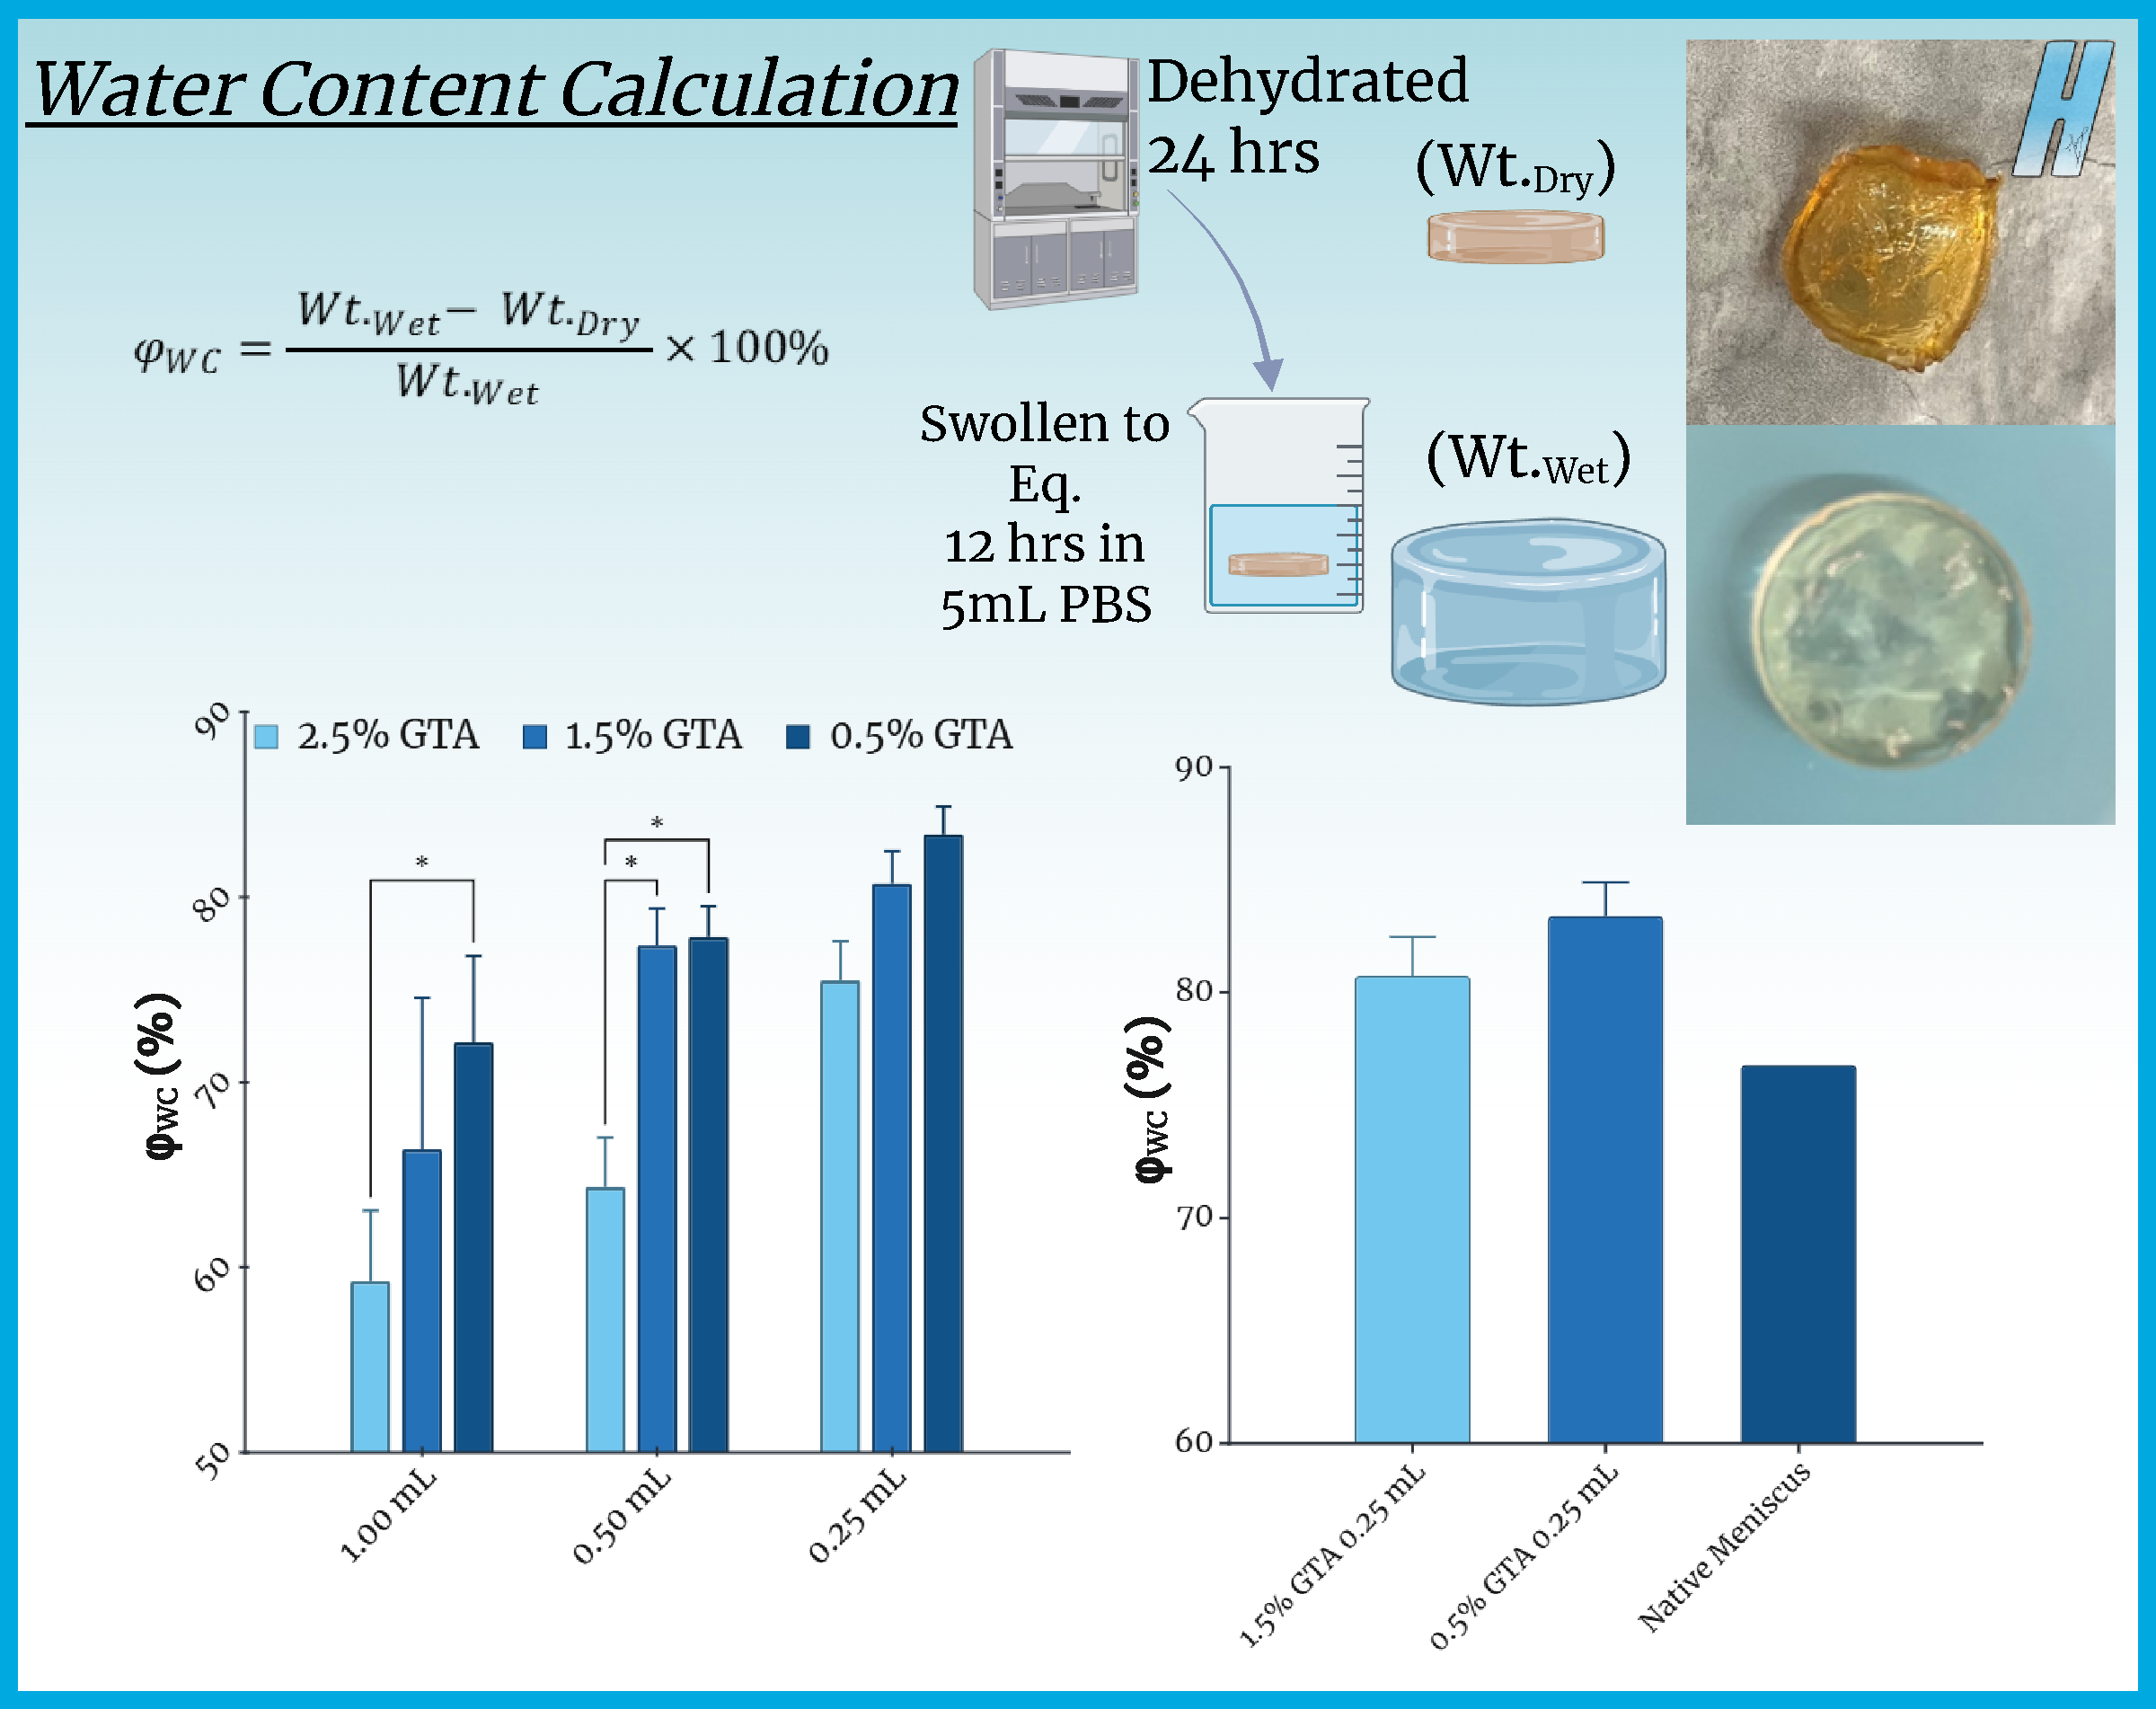
\includegraphics[width=1\linewidth]{figures/chapter 2/ch2_watercontent.pdf}
    \caption[Water Content Analysis of GelA--GTA Hydrogels.]{\textbf{Water Content Analysis of GelA--GTA Hydrogels.} Water content ($\varphi_{\mathrm{WC}}$) was calculated by comparing hydrated ($\mathrm{Wt}_{\mathrm{wet}}$) and dehydrated ($\mathrm{Wt}_{\mathrm{dry}}$) weights after equilibration in PBS and 24-hour drying. Representative images illustrate swollen and dehydrated hydrogels. The left graph shows $\varphi_{\mathrm{WC}}$ across varying GTA concentrations (0.5\%, 1.5\%, 2.5\% v/v) and crosslinker volumes (1.00, 0.50, 0.25 mL), highlighting the inverse relationship between crosslink density and hydration capacity (*$p < 0.05$). The right graph compares selected formulations (1.5\% GTA 0.25 mL and 0.5\% GTA 0.25 mL) to native meniscus tissue, demonstrating comparable water content to physiological levels.}
    \label{fig:ch2_watercontent}
\end{figure}

\subsection{Water Content Analysis}

The water content \((\phi_{WC})\) of GelA-GTA hydrogels was quantified across varying cross-linker concentrations and volumes to assess hydration properties critical for mimicking native meniscal tissue. As shown in Table~\ref{tab:ch2_water_content}, the water content decreased with increasing GTA concentration at each volume tested. Specifically, at 0.25~mL, hydrogels exhibited water contents of \(83.48\% \pm 5.99\%\), \(75.62\% \pm 5.49\%\), and \(80.85\% \pm 5.63\%\) for 0.5\%, 1.5\%, and 2.5\% GTA, respectively. Similarly, at 0.50~mL and 1.00~mL, a progressive reduction in \(\phi_{WC}\) was observed with increasing cross-linker concentration, indicating that higher GTA levels led to denser polymer networks and reduced hydration capacity. These results are consistent with prior findings highlighting the inverse relationship between cross-linking density and hydrogel swelling behavior.

\begin{table}[H]
    \centering
    \caption[Water Content Analysis]{\textbf{Water Content Analysis.} Measured water content (\%) across hydrogel formulations with varying crosslinker volumes (mL) and GTA concentrations (v/v), highlighting the relationship between crosslinking parameters and hydration capacity.}
    \label{tab:ch2_water_content}
    \renewcommand{\arraystretch}{1.3}
    \setlength{\tabcolsep}{12pt}
    \begin{tabular}{|p{3.5cm}|p{3.5cm}|p{3.5cm}|p{3.5cm}|}
        \hline
        \cellcolor{blue!20}\textbf{Water Content (\%)} & \multicolumn{3}{c|}{\cellcolor{blue!20}\textbf{GTA Concentrations (v/v)}} \\[0.3em]
        \hline
        \cellcolor{blue!20}\textbf{Volume (mL)} & \cellcolor{blue!20}\textbf{2.5\% GTA} & \cellcolor{blue!20}\textbf{1.5\% GTA} & \cellcolor{blue!20}\textbf{0.5\% GTA} \\[0.3em]
        \hline
        \cellcolor{blue!20}1.00 & 59.48 $\pm$ 4.54 & 67.54 $\pm$ 11.82 & 72.65 $\pm$ 9.71 \\[0.3em]
        \hline
        \cellcolor{blue!20}0.50 & 64.48 ± 4.07 & 77.49 ± 5.46 & 77.94 ± 4.93 \\[0.3em]
        \hline
        \cellcolor{blue!20}0.25 & 80.85 ± 5.63 & 75.62 ± 5.49 & 83.48 ± 5.99 \\[0.3em]
        \hline
    \end{tabular}
\end{table}



\subsection{Physiological Relevance}

Hydrogels intended for meniscal tissue engineering must closely replicate the high water content characteristic of native meniscal tissue, which has been reported as \(76.79\% \pm 3.32\%\)~\cite{morejon2020compressiveproperties}. Based on the measured water content (\(\phi_{WC}\)) of the fabricated hydrogel formulations, two specific crosslinking conditions were identified as optimal for further investigation:
\begin{itemize}
    \item 0.5\% GTA at 0.25 mL
    \item 1.5\% GTA at 0.25 mL
\end{itemize}

These two conditions provided water contents closest to physiological levels while preserving sufficient structural integrity necessary for subsequent mechanical testing. Moreover, it allowed for maintenance of a 10:1 vol/vol ratio for GelA--GTA solutions for future experiments~\cite{morejon2020compressiveproperties}.

Formulations crosslinked with 2.5\% GTA were excluded from further consideration due to excessive crosslinking, which resulted in significantly reduced water retention and compromised swelling behavior. Hydrogels crosslinked with 2.5\% GTA demonstrated markedly reduced water content, particularly at higher volumes, indicating excessive network densification that limited fluid uptake. This reduction in swelling behavior and water retention would likely compromise the viscoelastic behavior necessary for effective mechanical mimicry of the meniscus. Therefore, the 2.5\% GTA groups were not selected for further mechanical characterization.

Overall, selecting hydrogel formulations with physiological water content is critical to replicating the osmotic and load-bearing behaviors observed in native meniscal tissue, ensuring relevance for future mechanical testing and scaffold development.

\section{Mechanical Testing Challenges and Development of Novel Approaches}

Initial mechanical characterization of these hydrogel formulations presented several technical challenges that necessitated the development of specialized testing approaches. Traditional confined compression setups, while commonly used for biomaterial characterization, proved inadequate for accurately capturing the complex poroviscoelastic behavior of these highly hydrated constructs. Key limitations included poor force sensitivity at low strains and difficulties in maintaining sample hydration during extended testing periods. Additionally, challenges with platen alignment introduced measurement artifacts that compromised data accuracy. Furthermore, conventional testing geometries were poorly suited for detecting subtle differences between formulations, particularly during stress relaxation phases critical for assessing time-dependent mechanical responses. These limitations motivated the development of an improved testing apparatus, detailed in Chapter 3 (``Augmented via Additive''), which leverages additive manufacturing techniques to create custom-designed mechanical testing equipment specifically optimized for hydrogel characterization. This novel approach enables more precise measurement of mechanical properties while maintaining physiologically relevant testing conditions, ultimately providing deeper insights into the biomechanical behavior of these promising meniscal tissue engineering constructs.

\subsection{Mechanical Testing Protocol}

Testing was conducted using a custom-built confined compression apparatus with:

\begin{itemize}
    \item Temperature control (37$^\circ$C ± 0.5$^\circ$C)
    \item Hydration maintenance via PBS immersion
    \item Precise platen alignment (< 0.1$^\circ$ deviation)
    \item Real-time force and displacement monitoring
\end{itemize}

\section{"Hybrid" : Electrospun Gelatin Fibers} \label{sec:ch2_electrospinning}

\subsection{Co-Deposition with PCL Networks}

To enhance mechanical integrity and control scaffold porosity, an exploratory co-deposition method was developed. After electrospinning an initial 2~mL of the gelatin solution onto the collector plate, a pre-fabricated polycaprolactone (PCL) grid network was carefully placed on top of the partially formed fibrous mat. The remaining gelatin solution was then electrospun directly over the PCL network, effectively embedding the synthetic framework within the fibrous matrix.

The overarching purpose of this co-deposition strategy was to create composite constructs with **tunable porosity and integrated mechanical reinforcement, with the intent to later assess their permeability and integration potential within the overall HANI scaffold system. While mechanical testing was not conducted at this stage, these constructs were earmarked for future permeability assays designed to evaluate fluid transport properties critical for nutrient diffusion and tissue integration.

\subsection{Preliminary Observations}

SEM analysis confirmed the formation of randomly oriented fibers, successfully mimicking the superficial meniscal layer's disorganized collagen architecture. Fiber diameter was observed to increase with higher extrusion rates, consistent with prior findings~\cite{xie2009alignment}. Although the hybrid co-deposition technique was developed to improve mechanical integrity and porosity, further mechanical and permeability testing is required to validate its effectiveness.

\subsection{Electrospinning Chamber Refinements and Future Testing}

To facilitate improved fabrication control, a revised electrospinning chamber was developed utilizing custom-designed components produced via additive manufacturing. This refined setup aimed to improve environmental stability, precision alignment, and user safety during scaffold fabrication. Notably, the development of a custom permeation chamber, also fabricated using additive techniques, was initiated to evaluate the strain-dependent permeability of these co-deposition constructs. Details of the permeation chamber design, operational principles, and future testing protocols will be presented in Chapter~\ref{chap:3}, highlighting its role in assessing the fluid transport characteristics of HANI scaffold components.

\begin{figure}[H]
    \centering
    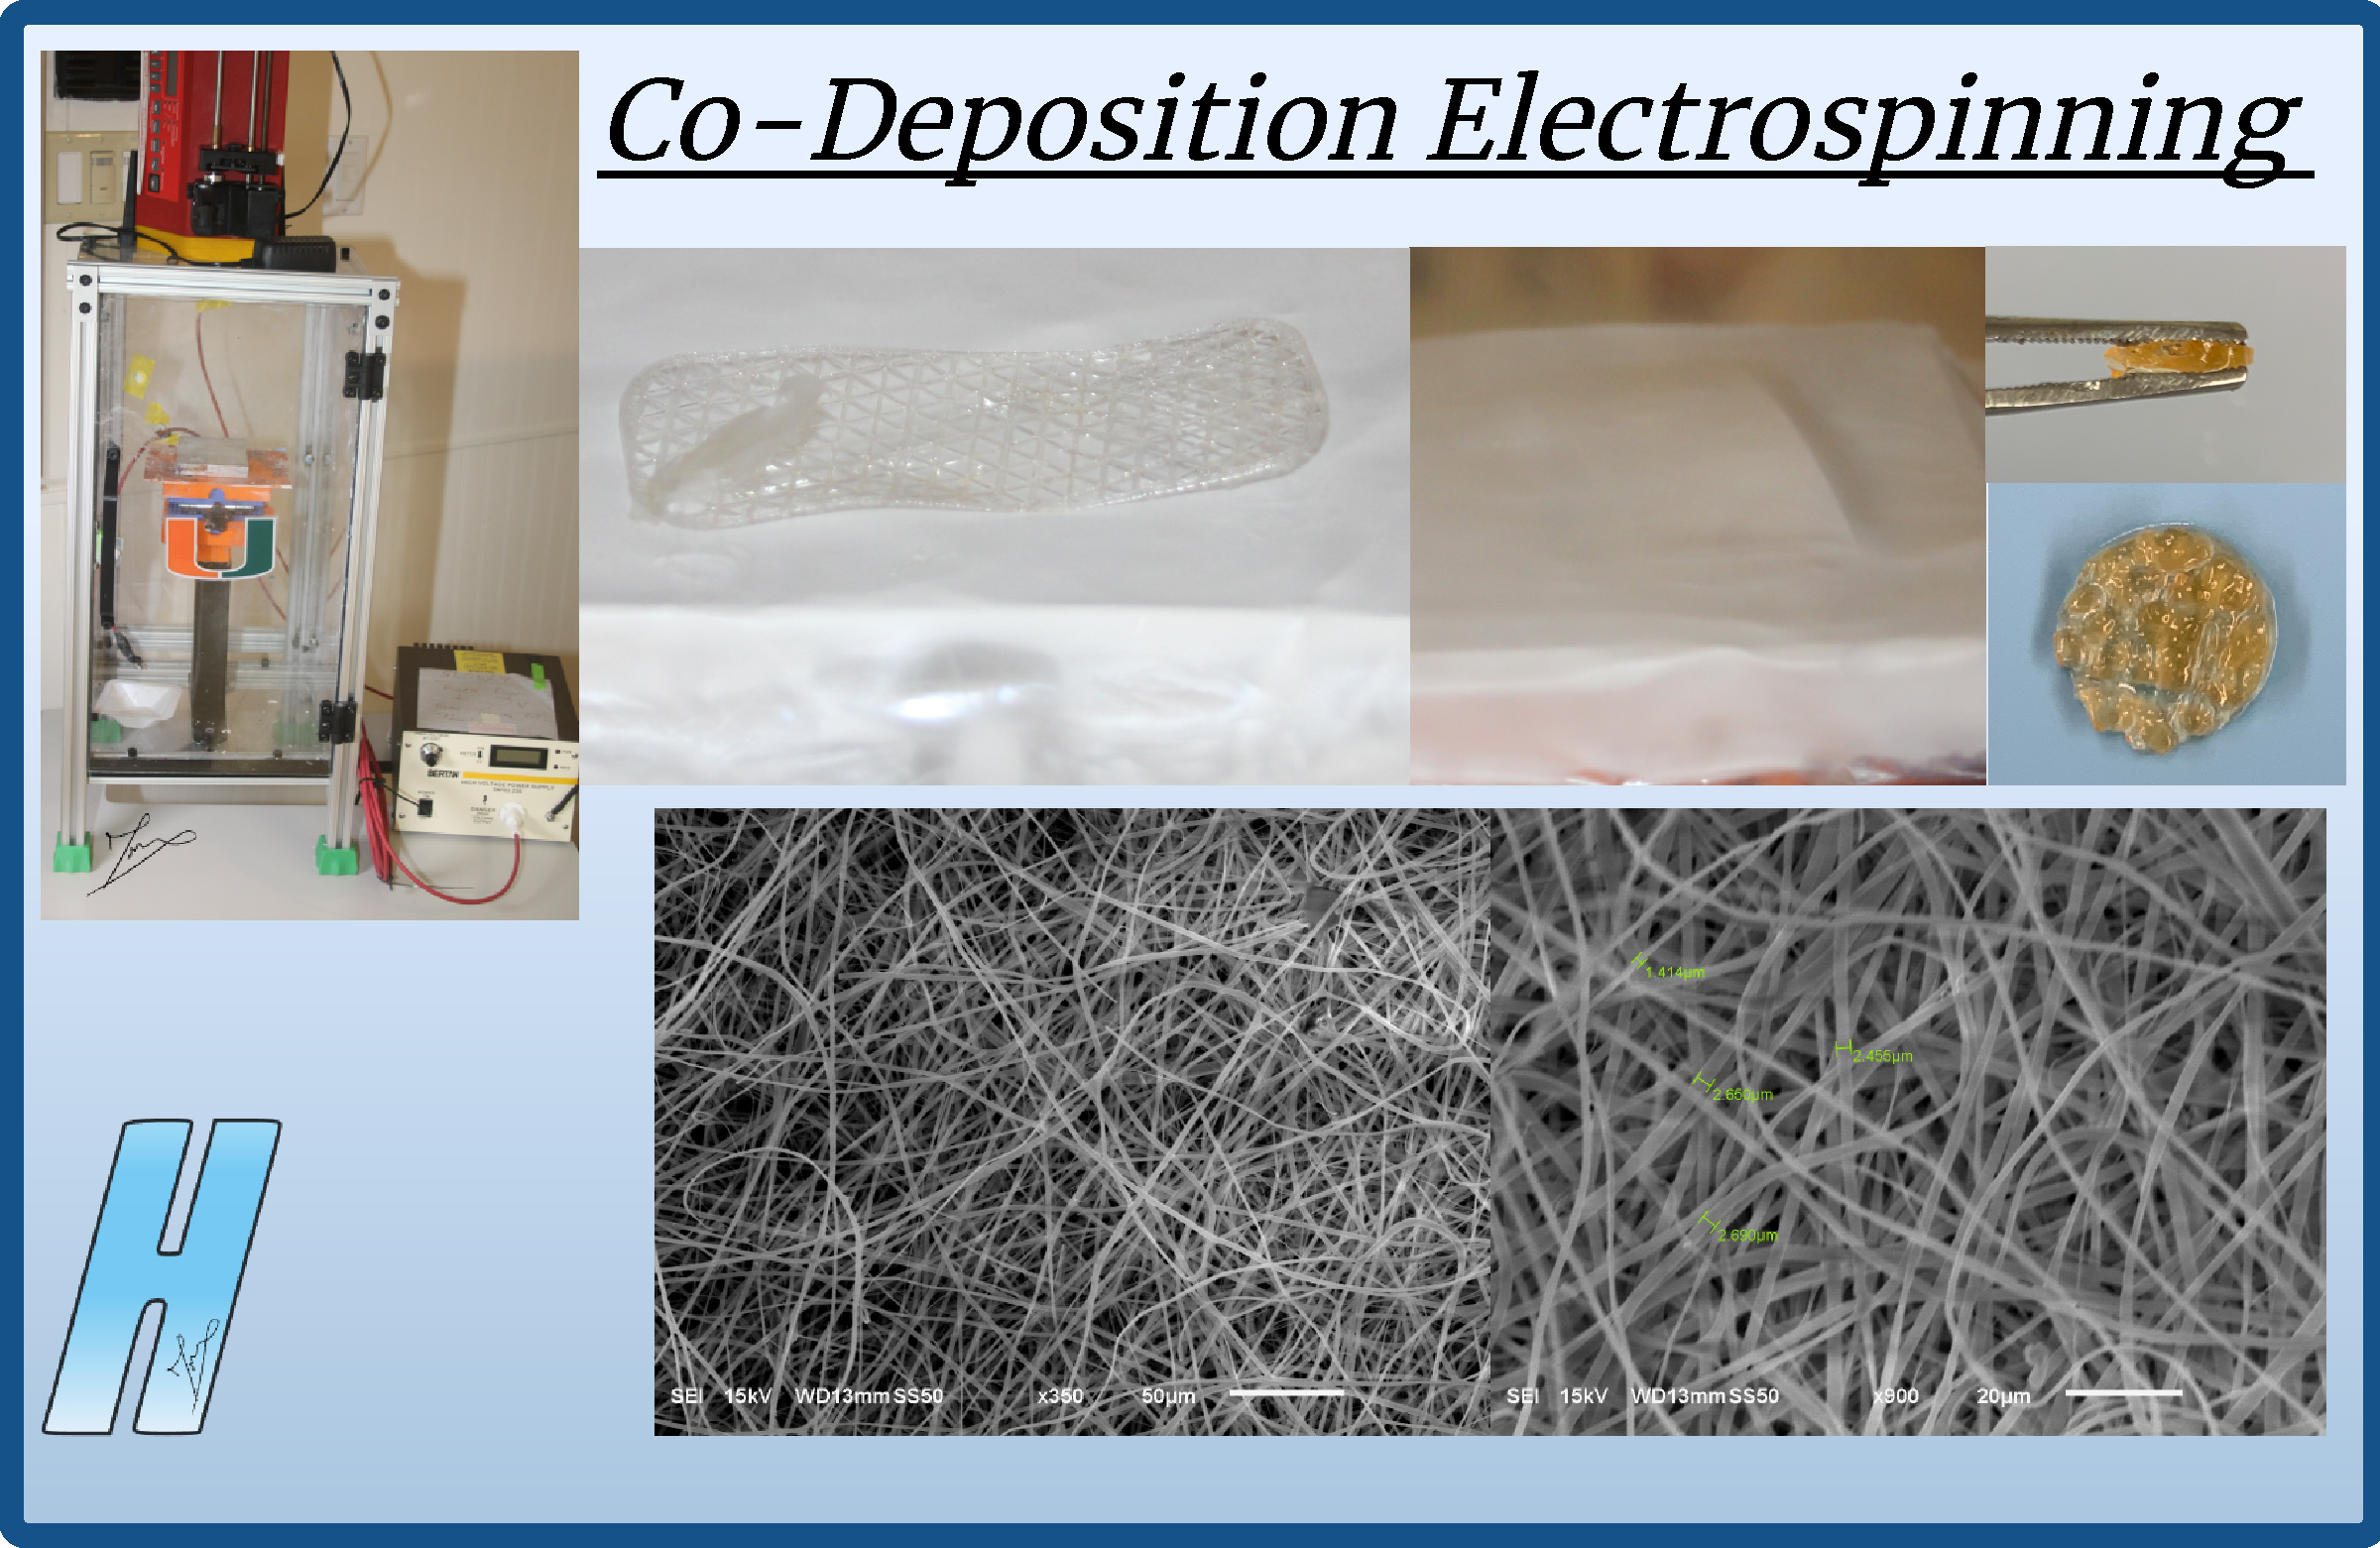
\includegraphics[width=0.8\textwidth]{figures/chapter 2/ch2_ES_sem.pdf}
    \caption[SEM Analysis of Scaffold Components.]{\textbf{SEM Analysis of Scaffold Components.} (A) Representative SEM image of electrospun gelatin fibers showing uniform fiber morphology and distribution. (B) SEM image of the PCL grid structure demonstrating the regular pattern and mechanical reinforcement properties. (C) Composite view showing the integration of gelatin fibers with the PCL grid structure. Scale bars represent 100~$\mu$m.}
    \label{fig:ch2_sem_analysis}
\end{figure}

\begin{table}[H]
    \centering
    \caption[Electrospinning Parameters and Conditions]{\textbf{Electrospinning Parameters and Conditions.} Detailed summary of key parameters and conditions used for gelatin fiber fabrication via electrospinning, including solution preparation, processing conditions, and post-treatment steps.}
    \label{tab:electrospinning_params}
    \renewcommand{\arraystretch}{1.3}
    \setlength{\tabcolsep}{12pt}
    \begin{tabular}{|p{4.5cm}|p{7.5cm}|}
        \hline
        \cellcolor{blue!20}\textbf{Parameter} & \cellcolor{blue!20}\textbf{Value / Description} \\
        \hline
        Polymer Solution & 10\% w/v Gelatin A in HFIP \\
        \hline
        Solvent & Hexafluoroisopropanol (HFIP) \\
        \hline
        Syringe & 10~mL Luer-lock \\
        \hline
        Dispensing Needle & 23G tip \\
        \hline
        Voltage & 21~kV \\
        \hline
        Flow Rate & 2 and 3~mL/hr \\
        \hline
        Needle-Collector Distance & 15~cm \\
        \hline
        Collector Type & Vertical aluminum block with foil \\
        \hline
        Crosslinking Agent & 2.5\% Glutaraldehyde (30~min) \\
        \hline
        Post-Treatment & Glycine rinse + DI water wash \\
        \hline
        Fiber Analysis & SEM imaging + diameter measurement \\
        \hline
        Co-Deposition Method & Initial 2~mL gelatin electrospun; PCL grid placed; remainder electrospun over \\
        \hline
    \end{tabular}
\end{table}

\clearpage

\section{Early ``HANI'' Scaffold Development}

Initial development of the Hybrid Hydrogels Augmented via Additive Network Integration (HANI) platform focused on the incorporation of poly-$\varepsilon$-caprolactone (PCL) reinforcement structures into gelatin-based hydrogel matrices. The goal was to fabricate composite scaffolds that exhibited improved mechanical strength and anisotropic characteristics aligned with the functional requirements of  the deep layer of native meniscal tissue. Early constructs featured PCL grids produced via fused deposition modeling (FDM), integrated directly into GelA--GTA hydrogels during the crosslinking process to promote cohesive bonding between the synthetic and hydrogel phases.

However, early mechanical testing exposed significant challenges. The compliant and hydrated nature of the hydrogels made compression testing difficult, with issues such as sample slippage, misalignment, and inconsistent force transmission limiting the reliability of initial data. These obstacles highlighted the need for a refined mechanical testing platform capable of delivering accurate, reproducible measurements.

In response, project efforts pivoted toward the iterative design and optimization of an enhanced confined compression system. This upgrade prioritized precise sample alignment, secure confinement, and seamless integration with imaging systems to facilitate high-resolution mechanical characterization. The testing platform improvements established a critical foundation for assessing scaffold poroviscoelastic properties and mechanical behavior under physiologically relevant loading.

A more detailed discussion of the additive manufacturing strategies and testing platform development will be presented in subsequent chapters: "A" (Augmented via Additive) and "ANI" (Additive Network Integration), where the engineering innovations and technical solutions are covered in depth.

\begin{figure}[H]
    \centering
    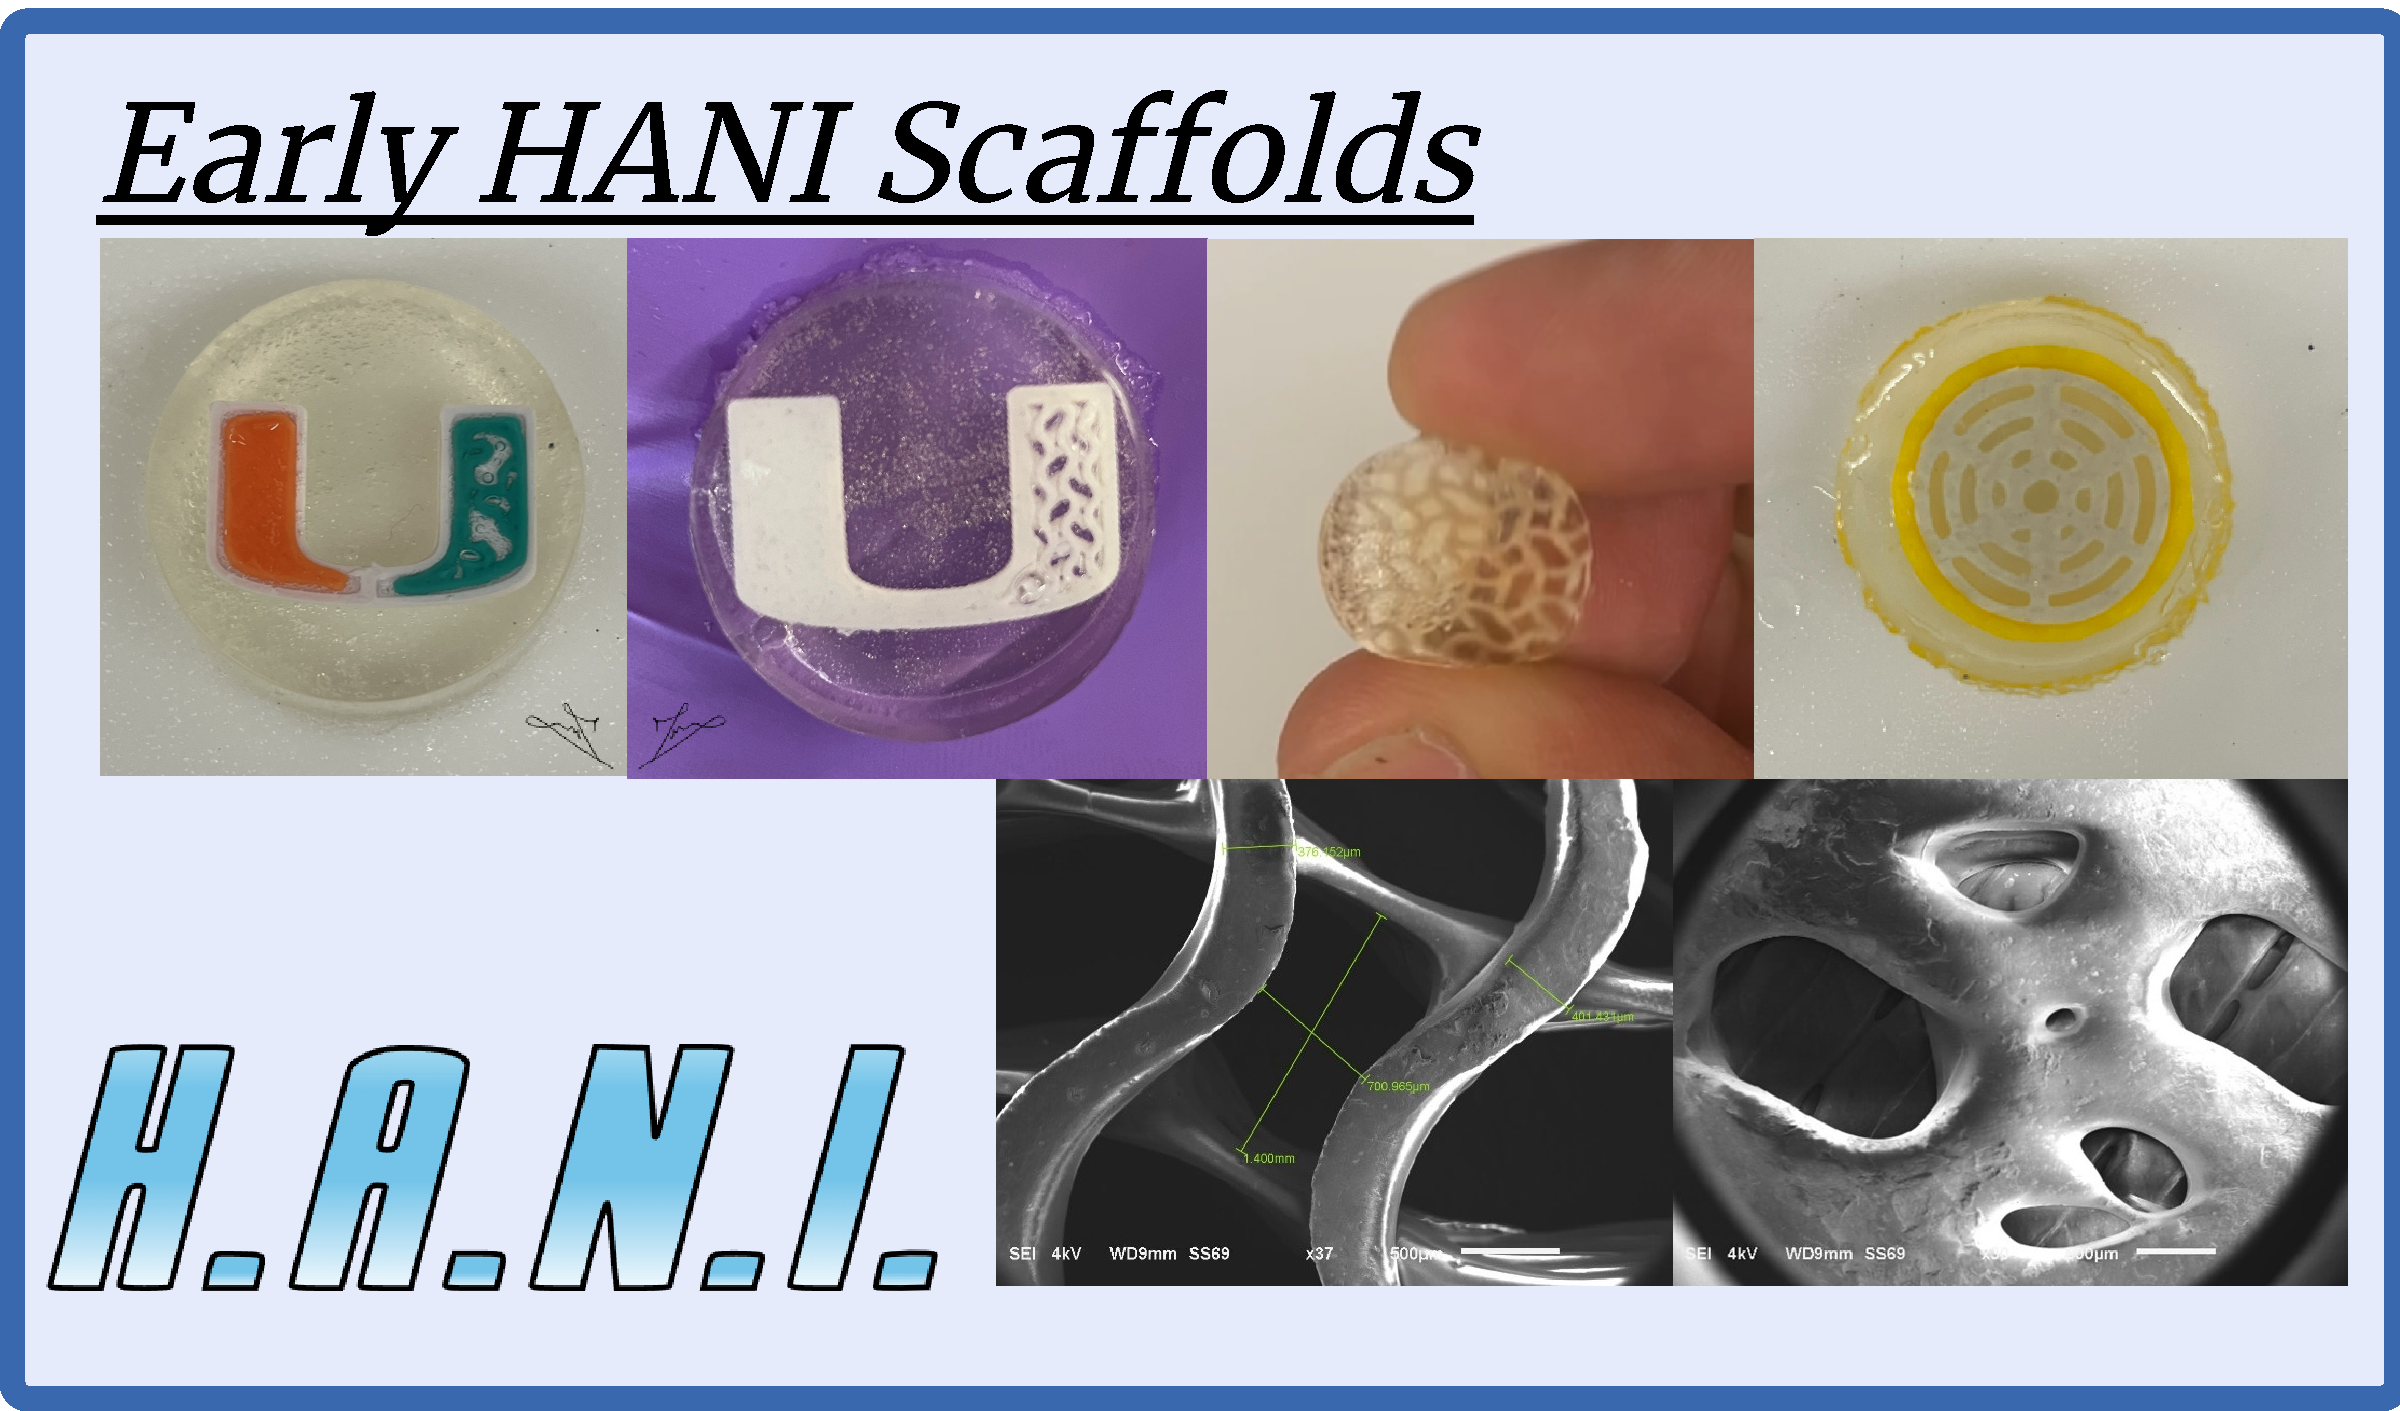
\includegraphics[width=0.8\textwidth]{figures/chapter 2/ch2_earlyHANI.pdf}
    \caption[Representative Early HANI Scaffold Prototype.]{\textbf{Representative Early HANI Scaffold Prototype.} (A) Top view of the prototype showing the integrated PCL grid structure within the gelatin matrix. (B) Side view demonstrating the layered architecture and thickness of the scaffold. (C) Close-up view highlighting the interface between the PCL reinforcement and gelatin matrix. Scale bars represent 1~mm.}
    \label{fig:ch2_earlyHANI}
\end{figure}


\section{Transitioning to Augmented via Additive}

The development and characterization of hybrid hydrogel systems presented in this chapter established a foundation for meniscal tissue engineering through GelA-GTA formulations. Our systematic investigation demonstrated the ability to achieve physiologically-relevant water content and swelling behavior while maintaining mechanical stability, particularly through the optimization of crosslinking parameters at 0.5\% and 1.5\% GTA concentrations with 0.25~mL volume. This platform enables precise control over:

\begin{itemize}
    \item Stress relaxation behavior through tunable crosslinking density and network architecture
    \item Mechanical properties via strategic GTA concentration and volume selection
    \item Dimensional control and geometric precision through standardized fabrication protocols
    \item Swelling kinetics and equilibrium water content for physiological relevance
\end{itemize}

However, the characterization process revealed significant limitations in conventional mechanical testing approaches for these highly hydrated constructs. Traditional confined compression setups proved inadequate for capturing the complex poroviscoelastic behavior critical to meniscal function. These challenges, including poor force sensitivity, hydration maintenance issues, and alignment difficulties, highlight the need for more sophisticated testing methodologies.

Chapter 3, "Augmented via Additive," builds upon these findings by introducing novel instrumentation specifically designed to capture the complex poroviscoelastic behavior of these promising scaffold materials. Through the integration of additive manufacturing techniques, we develop custom-designed mechanical testing equipment optimized for hydrogel characterization, enabling more precise measurement of mechanical properties while maintaining physiologically relevant testing conditions.
